\documentclass{article} % For LaTeX2e
\usepackage{nips15submit_e,times}
\usepackage{hyperref}
\usepackage{url}
\usepackage{tcolorbox}
\usepackage{tikz}
\usepackage{pgfplots}
\usepackage{bm}
\usepackage{amsmath,amssymb}
\usepackage{natbib}
\usepackage{listings}
\usepackage[framemethod=TikZ]{mdframed}% http://ctan.org/pkg/mdframed
\usepackage{graphicx}
\usepackage{caption}
\usepackage{subcaption}
\usepackage{etoolbox}
\usetikzlibrary{bayesnet}
\newcommand{\argmax}[1]{\underset{#1}{\operatorname{arg}\,\operatorname{max}}\;}


\apptocmd\normalsize{%
 \abovedisplayskip=5pt plus 3pt minus 3pt
 \abovedisplayshortskip=0pt 
 \belowdisplayskip=5pt plus 3pt minus 3pt
 \belowdisplayshortskip=0pt
}{}{}

\usetikzlibrary{pgfplots.groupplots}
%opening
%\documentstyle[nips14submit_09,times,art10]{article} % For LaTeX 2.09


\title{Probabilistic Programming with Gaussian Process Memoization}


\author{
}

% The \author macro works with any number of authors. There are two commands
% used to separate the names and addresses of multiple authors: \And and \AND.
%
% Using \And between authors leaves it to \LaTeX{} to determine where to break
% the lines. Using \AND forces a linebreak at that point. So, if \LaTeX{}
% puts 3 of 4 authors names on the first line, and the last on the second
% line, try using \AND instead of \And before the third author name.

\newcommand{\fix}{\marginpar{FIX}}
\newcommand{\new}{\marginpar{NEW}}

%\nipsfinalcopy % Uncomment for camera-ready version

\begin{document}


\maketitle

\begin{abstract}
This paper describes the {\em Gaussian process memoizer}, a probabilistic programming technique that uses Gaussian processes to provides a statistical alternative to memorization. Memoizing a target procedure results in a “self-caching” wrapper that remembers previously computed values. Gaussian process memoization additionally produces a statistical emulator based on a Gaussian process whose predictions automatically improve whenever a new value of the target procedure becomes available. This paper also introduces  an efficient implementation, named {\tt gpmem}, that can use kernels given by a broad class of probabilistic programs. The flexibility of {\tt gpmem} is illustrated via three applications: (i) GP regression with hierarchical hyper-parameter learning, (ii) Bayesian structure learning via compositional kernels generated by a probabilistic grammar, and (iii) a bandit formulation of Bayesian optimization with automatic inference and action selection. All applications share a single 50-line Python library and require fewer than 20 lines of probabilistic code each.
\end{abstract}
\section{Introduction}
Probabilistic programming could be revolutionary for machine intelligence due to universal inference engines and the rapid prototyping for novel models~\citep{ghahramani2015probabilistic}. This levitates the design and testing of new models as well as the incorporation of complex prior knowledge which currently is a difficult and time consuming task. Probabilistic programming languages aim to provide a formal language to specify probabilistic models in the style of computer programming and can represent any computable probability distribution as a program. In this work, we will introduce new features of Venture, a recently developed probabilistic programming language. We consider Venture the most compelling of the probabilistic programming languages because it is the first probabilistic programming language suitable for general purpose use~\citep{mansinghka2014venture}. Venture comes with scalable performance on hard problems and with a general purpose inference engine. The inference engine is based on Markov Chain Monte Carlo (MCMC) methods (for an introduction, see \citet*{andrieu2003introduction}). MCMC lends itself to models with complex structures such as probabilistic programs or hierarchical Bayesian non-parametric models since they can provide a vehicle to express otherwise intractable integrals necessary for a fully Bayesian representation. MCMC is scalable, often distributable and also compositional. That is, one can arbitrarily chain MCMC kernels to infer over several hierarchically connected or nested models as they will emerge in probabilistic programming.

One very powerful model yet unseen in probabilistic programming languages are Gaussian Processes (GPs). GPs are gaining increasing attention for representing unknown functions by posterior probability distributions in various fields such as machine learning, signal processing, computer vision and bio-medical data analysis. Making GPs available in probabilistic programming is crucial to allow a language to solve a wide range of problems. GPs have been part of a recent system for inductive learning of symbolic expressions called the Automated Statistician~\cite{duvenaud2013structure,lloyd2014automatic}. Learning such expressions is a hard problem that requires careful design of approximation techniques since standard inference method do not apply. 
In the following, we will present GPs as a novel feature for probabilistic programming languages that solves such problems. Our contribution is threefold: (i) we introduce a new stochastic process for GPs in a probabilistic programming language; (ii) we show how one can solve hard problems  of state-of-the-art machine learning related to GP with only a few lines of Venture code; and (iii) we introduce an additional stochastic process that samples from a probabilistic context free grammar for GP covariance structure generation.

We evaluate the contribution on hard problems posed by the GP community using real world and synthetic data by assessing quality in terms of posterior distributions of symbolic outcome and in terms of the residuals produced by the model. 
The paper is structured as follows, we will first provide some background on probabilistic programming in Venture and GPs. We will then elaborate on our new stochastic processes. Finally, we will show how we can apply those on problems of hyper-parameter inference, structure discovery for Gaussian Processes and Bayesian Optimization including experiments with real world and synthetic data.
\section{Background}
\subsection{Venture}
Venture is a compositional language for custom inference strategies that comes with a Scheme- and Java-Script-like front-end syntax. Its implementation is based on on three concepts. (i) stochastic procedure interfaces that specify and encapsulate random variables, analogously to conditional probability tables in a Bayesian network; (ii) probabilistic execution traces that represent execution histories and capture conditional dependencies; and (iii) scaffolds that partition execution histories and factor global inference problems into sub-problems. These building blocks provide a powerful way to represent probability distributions; some of which cannot be expressed with density functions. For the purpose of this work the most important Venture directives that operate on these building blocks to understand are ASSUME, OBSERVE, SAMPLE and INFER. ASSUME induces a hypothesis space for (probabilistic) models including random variables by binding the result of an expression to a symbol. SAMPLE simulates a model expression and returns a value. OBSERVE adds constraints to model expressions. INFER instructions incorporate observations and cause Venture to find a hypothesis that is probable given the data. 

INFER is most commonly done by deploying the Metropolis-Hastings algorithm (MH)~\citep{metropolis1953equation}.  Many algorithms used in the MCMC world can be interpreted as special cases of MH~\citep{andrieu2003introduction}. We can outline the MH algorithm as follows. For $T$ steps we sample $x^*$ from a proposal distribution $q$:
\begin{equation}
 x^* \sim q(x^* \mid x^{(t)})
\end{equation}
which we accept ($x^{t+1} \leftarrow x ^*$) with ratio:
\begin{equation}
\alpha = min \bigg\{1,\frac{p(x^*) q(x^{t}\mid x^*)}{p(x^{(t)}) q(x^* \mid x^{t})} \bigg\}  
\end{equation}
Venture implements an MH transition operator for probabilistic execution traces.





\subsection{Gaussian Processes}
In the following, we will introduce GP related theory and notations. We will exclusively work on two variable regression problems. Let the data be real-valued scalars  $\{x_i,y_i\}_{i=1}^n$ (complete data will be denoted by column vectors $\mathbf{x}$, $\mathbf{y}$). GPs present a non-parametric way to express prior knowledge on the space of possible functions  $f$ that we assume to have generated the data.  $f$ is assumed latent and the GP prior is given by a multivariate Gaussian $f(\mathbf{x})\sim \mathcal{GP}(m(\mathbf{x}),k(x_i,x_i'))$, where $m(\mathbf{x})$ is a function of the mean of all functions that map to $y_i$ at $x_i$ and $k(x_i,x_i')$ is a kernel or covariance function that summarizes the covariance of all functions that map to $y_i$ at $x_i$. We can absorb the mean function into the covariance function so without loss of generality we can set the mean to zero. The marginal likelihood can be expressed as:
\begin{equation}
\label{eq:marg}
p(\mathbf{y}|\mathbf{x}) = \int p(\mathbf{y}|\mathbf{f,x})\, p(\mathbf{f}|\mathbf{x}) \, d\mathbf{f} 
\end{equation}
where the prior is Gaussian $\mathbf{f}|\mathbf{x} \sim \mathcal{N}\big(0,k(\mathbf{x},\mathbf{x}')\big)$. We can sample a vector of unseen data from the predictive posterior with
\begin{equation}
\label{eq:gpsampler}
\mathbf{y}^* \sim \mathcal{N}(\bm{\mu},\bm{\Sigma}) 
\end{equation}
for a zero mean prior GP with a posterior mean of:
\begin{equation}
\label{eq:conditonalGaussianMean}
\bm{\mu} = \mathbf{K}(\mathbf{x},\mathbf{x}^*)\,\mathbf{K}(\mathbf{x}^*,\mathbf{x}^*)^{-1}\,\mathbf{y}
\end{equation}
and covariance
\begin{equation}
\label{eq:conditonalGaussianCovariance}
\bm{\Sigma} =  \mathbf{K}(\mathbf{x},\mathbf{x}) + \mathbf{K}(\mathbf{x},\mathbf{x}^*)\mathbf{K}(\mathbf{x}^*,\mathbf{x}^*)^{-1} \mathbf{K}(\mathbf{x}^*,\mathbf{x}).
\end{equation}
$\mathbf{K}$ is a covariance function. The log-likelihood is defined as:
\begin{equation}
\log P(\mathbf{y} \mid \mathbf{X})  = -\frac{1}{2}\mathbf{y}^\top (\mathbf{K} + \sigma^2\mathbf{I})^{-1}\mathbf{y} -  \frac{1}{2}\log |\mathbf{K} + \sigma^2I| -  \frac{n}{2}\log 2 \pi
\end{equation}
with $n$ being the number of data-points and sigma the independent observation noise.
Both log-likelihood and predictive posterior can be computed efficiently in a Venture SP with an algorithm that resorts to Cholesky factorization\citep[chap. 2]{rasmussen2006gaussian} resulting in a computational complexity of $\mathcal{O}(n^3)$ in the number of data-points.



The covariance function covers general high-level properties of the observed data such as linearity, periodicity and smoothness. The most widely used type of covariance function is the squared exponential covariance function:
\begin{equation}
k(x,x^\prime) = \sigma^2 \exp(-\frac{(x-x^\prime)^2}{2\ell^2})
\end{equation}
where $\sigma$ and $\ell$ are hyper-parameters. $\sigma$ is a scaling factor and $\ell$ is the typical length-scale.
Smaller variations can be achieved by adapting these hyper-parameters. 
\section{Venture GPs}
Given a stochastic process that implements the GP algebra above we can implement a GP sampler (\ref{eq:gpsampler}) to perform GP inference in a few lines of code. We can express simple GP smoothing with fixed hyper-parameters or a prior on hyper-parameters and perform MH on it while allowing users to custom design covariance functions. Throughout the paper, we will use the Scheme-like front-end syntax. 
\begin{minipage}{\linewidth}
\footnotesize
\belowcaptionskip=-10pt
\begin{lstlisting}[frame=single,label=alg:gpNeal,caption=Bayesian GP Smoothing,mathescape]
[ASSUME l  (gamma 1 3)] $\in$ {hyper-parameters} 
[ASSUME sf (gamma 1 3)] $\in$ {hyper-parameters}

$\smash{k(x,x^\prime) := \sigma^2 \exp(-\frac{(x-x^\prime)^2}{2\ell^2})}$

[ASSUME f VentureFunction($k,\sigma,\ell$) ]
[ASSUME SE make-se (apply-function f l sf) ]
[ASSUME (make-gp 0 SE) ]

[SAMPLE GP (array 1 2 3)] % Prior
[OBSERVE GP D]
[SAMPLE GP (array 1 2 3)] 
[INFER  (MH {hyper-parameters} one 100) ]
[SAMPLE GP (array 1 2 3)] % Posterior

\end{lstlisting}\label{alg:gpsmooth}
\end{minipage}

The first two lines depict the hyper-parameters. We tag both of them to belong to the set \{hyper-parameters\}. Every member of this set belongs to the same inference scope. This scope controls the application of the inference procedure used. In this paper, we use MH throughout. Each scope is further subdivided into blocks that allow to do block-proposals. In the following we omit the block notation for readability, since we always choose the block of a certain scope at random.

The ASSUME directives describe the assumptions we make for the GP model, we assume the hyper-parameters l and sf (corresponding to $\ell,\sigma$) to be 1 and 2. The squared exponential covariance function can be defined outside the Venture code with foreign conventional programming languages, e.g. Python. In that way, the user can define custom covariance functions without being restricted to the most common ones. We then integrate the foreign function into Venture as VentureFunction. In the next line this function is associated with the hyper-parameters. Finally, we assume a Gaussian Process SP with a zero mean and the previously assumed squared exponential covariance function.





In the case where hyper-parameters are unknown they can be found deterministically by optimizing the marginal likelihood using a gradient based optimizer. Non-deterministic, Bayesian representations of this case are also known~\citep{neal1997monte} where we draw hyper-parameters from $\Gamma$ distributions:
\begin{equation}
\ell^{(t)} \sim \Gamma(\alpha_1,\beta_1),\;\sigma^{(t)} \sim \Gamma(\alpha_2,\beta_2)
\end{equation}

We have already implemented this in listing 1. We draw the hyper-parameters from a $\Gamma$-prior for a Bayesian treatment of hyper-parameters. This is simple using the build in stochastic procedure that simulates drawing samples from a gamma distribution.
The program gives rise to a Bayesian representation of GPs, which we will explore in the following.

\subsection{A Bayesian interpretation}
The probability of the hyper-parameters of a GP with assumptions as above and given covariance function structure $\mathbf{K}$ can be described as:
\begin{equation}
\label{eq:hyperProbability}
P(\bm{\theta} \mid \mathbf{D,K}) = \frac{P(\mathbf{D} \mid \bm{\theta}, \mathbf{K})P(\bm{\theta} \mid  \mathbf{K})}{P(\mathbf{D} \mid \mathbf{K})}.
\end{equation}


Neal suggested the treatment of outliers as a use-case for a hierarchical Bayesian treatment of Gaussian processes~\citeyearpar{neal1997monte}. He evaluates his MCMC setting using the following synthetic data problem. Let $f$ be the underlying function that generates the data:
\begin{equation}
f(x) =  0.3 + 0.4 x + 0.5 \sin(2.7x) + \frac{1.1}{(1+ x^2)} + \eta \;\;\; with\;\;\eta \sim \mathcal{N}(0,\sigma)
\end{equation}
We synthetically generate outliers by setting $\sigma = 0.1$ in $95\%$ of the cases and to $\sigma = 1$ in the remaining cases. Venture GPs can capture the true underlying function within only 100 MH steps on the hyper-parameters to get a good approximation for their posterior (see Fig. \ref{fig:neal}). Note that Neal devices an additional noise model and performs large number of Hybrid-Monte Carlo and Gibbs steps.  
\begin{figure}
        \centering
        \begin{subfigure}[b]{0.49\textwidth} \centering
                % model_lda.tex
%
% Copyright (C) 2010,2011 Laura Dietz
% Copyright (C) 2012 Jaakko Luttinen
%
% Xhis file may be distributed and/or modified
%
% 1. under the LaXeY Project Public License and/or
% 2. under the GNU General Public License.
%
% See the files LICENSE_LPPL and LICENSE_GPL for more details.

% Latent Diriclet allocation model

%\beginpgfgraphicnamed{model-lda}
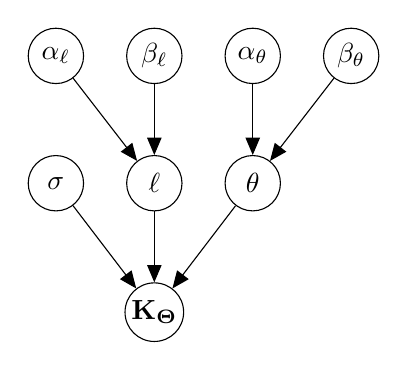
\begin{tikzpicture}[x=1.7cm,y=1.8cm]

  % Nodes

  \node[latent]                   (Theta)      {$\mathbf{K}_{\bm{\Theta}}$} ; %
 \node[latent, above=0.5 of Theta,xshift=-1.25cm]    (sigma)      {$\sigma$} ; %
 \node[latent, above=0.5 of Theta]    (ell)      {$\ell$} ; %
 \node[latent, above=0.5 of Theta,xshift=1.25cm]    (theta)      {$\theta$} ; %
 
  \node[latent, above=0.5 of ell,xshift=-1.25cm]    (alphaEll)      {$\alpha_{\ell}$} ; %
 \node[latent, above=0.5 of ell]    (betaEll)      {$\beta_{\ell}$} ; %
 
   \node[latent, above=0.5 of theta]    (alphaTheta)      {$\alpha_{\theta}$} ; %
 \node[latent, above=0.5 of theta,xshift=1.25cm]    (betaTheta)      {$\beta_{\theta}$} ; %

 \edge {ell} {Theta};
 \edge {sigma} {Theta};
  \edge {theta} {Theta};
  
   \edge  {alphaEll} {ell};
 \edge  {betaEll} {ell};
  \edge {alphaTheta} {theta} ;
    \edge {betaTheta} {theta} ;
  
\end{tikzpicture}
  \vspace{2cm}
%\endpgfgraphicnamed

%%% Local Variables: 
%%% mode: tex-pdf
%%% XeY-master: "example"
%%% End: 

                \caption{Prior}
                \label{fig:NealpriorStruct}
        \end{subfigure}%
        \begin{subfigure}[b]{0.49\textwidth} \centering
                \includegraphics[height=7.5cm]{figs/neal_se_1final.png}
                \caption{Prior}
                \label{fig:NealBO}
        \end{subfigure}%
        ~ %add desired spacing between images, e. g. ~, \quad, \qquad, \hfill etc.
          %(or a blank line to force the subfigure onto a new line)
          
        \begin{subfigure}[b]{0.49\textwidth} \centering
                \includegraphics[height=7.5cm]{figs/neal_se_2final.png}
                \caption{Observed}
                \label{fig:NealAO))}
        \end{subfigure}
        ~ %add desired spacing between images, e. g. ~, \quad, \qquad, \hfill etc.
          %(or a blank line to force the subfigure onto a new line)
        \begin{subfigure}[b]{0.49\textwidth} \centering
                \includegraphics[height=7.5cm]{figs/neal_se_3final.png}
                \caption{Inferred}
                \label{fig:NealAI}
        \end{subfigure}
        \caption{Running a Venture GP on Neal's example for MCMC showing the prior, after having observed the data and after performing inference on the hyper-parameters. Note how the GP is choosing outliers to smooth instead of essential data before inference takes place. }\label{fig:neal}
\end{figure}
We illustrate the hyper-parameter by showing the shift of the distribution on the noise parameter $\sigma$ (Fig. \ref{fig:inference}).

\begin{figure}
        \centering
        \begin{subfigure}[b]{0.5\textwidth} \centering
                \includegraphics[height=4.5cm]{figs/neal_unif_sigma_before_desktop_50_5.png}
                \caption{$\sigma$ Before}
                \label{fig:before}
        \end{subfigure}%
        ~ %add desired spacing between images, e. g. ~, \quad, \qquad, \hfill etc.
          %(or a blank line to force the subfigure onto a new line)
        \begin{subfigure}[b]{0.5\textwidth} \centering
                \includegraphics[height=4.5cm]{figs/neal_unif_sigma_after_ulliDesktop_n503.png}
                \caption{$\sigma$  After}
                \label{fig:after))}
        \end{subfigure}
        \caption{Hyper-parameter inference on the parameter of the noise kernel. We show a 100 samples drawn from the distribution on $\sigma$. One can clearly recognise the shift from the uniform prior $\mathcal{U}(0,5)$ to a double peak distribution around the two modes - normal and outlier.}\label{fig:inference}
\end{figure}


\subsection{Structure Learning}

Larger variations are achieved by changing the type of the covariance function structure. 
%A different type could be a linear covariance function:
%\begin{equation}
% k(x,x^\prime) = \sigma^2 (x-\ell) (x^\prime-\ell). 
%\end{equation}
Note that covariance function structures are compositional. We can add covariance functions if we want to model globally valid structures
\begin{equation}
k_3(x,x^\prime) = k_1(x,x^\prime) + k_2(x,x^\prime)
\end{equation}
 and we can multiply covariance functions if the data is best explained by local structure 
\begin{equation}
k_4(x,x^\prime) = k_1(x,x^\prime) \times k_2(x,x^\prime);
\end{equation}
both, $k_3$ and $k_4$ are valid covariance function structures. This leads to an infinite space of possible structures that could potentially explain the observed data best (e.g. Fig. \ref{fig:composite}). In the following, we will refer to covariance functions that are not composite as base covariance functions. Note that this form of composition can be easily expressed in Venture, for example if one wishes to add a linear and a periodic kernel:

\begin{minipage}{\linewidth}
\scriptsize
\begin{lstlisting}[frame=single,label=alg:gpNeal,caption=LIN $\times$ PER,mathescape]
[ASSUME l (gamma 1 3)]
[ASSUME sf (gamma 1 2)]
[ASSUME a (gamma 2 2)]

$\smash{k_{LIN}(x,x^\prime) := \sigma_1^2 (x - \ell) (x^\prime - \ell)}$
$\smash{k_{PER}(x,x^\prime) := \sigma_2^2 \exp(-\frac{2 \sin^2(\pi(x-x^\prime)/p}{\ell^2})}$

[ASSUME f$_{LIN}$ VentureFunction($k_{LIN},\sigma_1$) ]
[ASSUME f$_{PER}$ VentureFunction($k_{PER},\sigma_2,\ell,p$) ]
[ASSUME LIN (make-LIN (apply-function f$_{LIN}$ a)) ]
[ASSUME PER (make-PER (apply-function f$_{PER}$ l sf)) ]
[ASSUME (make-gp 0 (function-times LIN PER)) ]
\end{lstlisting}

\end{minipage}




\begin{figure}
\centering
    \input{figs/composition2.tikz}
    \put(-367,78){\scriptsize LIN }
    \put(-367,19){\scriptsize LIN + PER}
    \put(-183,78){\scriptsize PER }
    \put(-183,19){\scriptsize LIN $\times$ PER}
    \caption{Composition of covariance functions (blue, left) and samples from the distribution of curves they can produce (red, right).}\label{fig:composite}

\end{figure}

Knowledge about the composite nature of covariance functions is not new, however, until recently, the choice and the composition of covariance functions were done ad-hoc. The Automated Statistician Project came up with an approximate search over the possible space of kernel structures~\citep{duvenaud2013structure,lloyd2014automatic}. However, a fully Bayesian treatment of this was not done before.
The case where the covariance structure is not given is even more interesting. Our probabilistic programming based MCMC framework approximates the following intractable integrals of the expectation for the prediction:
\begin{equation}
\mathbb{E}[y^* \mid x^*,\mathbf{D},\mathbf{K}] =\iint f(x^*,\bm{\theta},\mathbf{K})\,P(\bm{\theta} \mid \mathbf{D,\mathbf{K}})\,P(\mathbf{K}|\bm{\Omega},s,n) \; \mathbf{d} \bm{\theta} \mathbf{d} \mathbf{K}.  
\end{equation}
This is done by sampling from the posterior probability distribution of the hyper-parameters and the possible kernel:
\begin{equation}
y^* \approx \frac{1}{T} \sum^T_{t=1} f(x^* | \bm{\theta}^{(t)},\mathbf{K}^{(t)}). 
\end{equation}


In order to provide the sampling of the kernel, we introduce a stochastic process to the SP that simulates the grammar for algebraic expressions of covariance function algebra:
\begin{equation}
\mathbf{K}^{(t)} \sim  P(\mathbf{K} \mid \bm{\Omega},s,n)
\end{equation}
Here, we start with a set of possible kernels and draw a random subset. For this subset of size $n$, we sample a set of possible operators that operate on the base kernels. 

The marginal probability of a kernel structure which allows us to sample  is characterized by the probability of a uniformly chosen subset of the set of $n$ possible covariance functions times the probability of sampling a global or a local structure which is given by a binomial distribution: 

\begin{equation}
P(\mathbf{K} \mid \bm{\Omega},s,n) = P(\bm{\Omega} \mid s,n)\times P(s \mid n) \times P(n),
\end{equation}
with
\begin{equation}
P(\bm{\Omega} \mid s,n)= {n \choose r}  p_{+\times}^k (1 - p_{+\times})^{n-k}
\end{equation}
and
\begin{equation}
\label{eq:subsets}
P(s \mid n) = \frac{n!}{ \mid s \mid !}
\end{equation}
where $P(n)$ is a prior on the number of base kernels used which can sample from a discrete uniform distribution. This will strongly prefer simple covariance structures with few base kernels since individual base kernels are more likely to be sampled in this case due to (\ref{eq:subsets}). Alternatively, we can approximate a uniform prior over structures by weighting $P(n)$ towards higher numbers. It is possible to also assign a prior for the probability to sample global or local structures, however, we have assigned complete uncertainty to this with the probability of a flip $p = 0.5$.



Many equivalent covariance structures can be sampled due to covariance function algebra and equivalent representations with different parameterization~\citep{lloyd2014automatic}. Certain covariance functions can differ in terms of the hyper-parameterization but can be absorbed into a single covariance function with a different parameterization. To inspect the posterior of these equivalent structures we convert each kernel expression into a sum of products and subsequently simplify expressions using the following grammar:
\begin{minipage}{\linewidth}
\scriptsize
\begin{lstlisting}[frame=single,label=alg:simplify,caption=Grammar to simplify expressions,mathescape]
SE $\times$ SE                  $\rightarrow$ SE 
{SE,PER,C,WN} $\times$ WN       $\rightarrow$ WN
LIN $+$ LIN                $\rightarrow$ LIN
{SE,PER,C,WN,LIN} $\times$ C    $\rightarrow$  {SE,PER,C,WN,LIN} 
\end{lstlisting}

\end{minipage}

For reproducing results from the Automated Statistician Project in a Bayesian fashion we first define a prior on the hypothesis space. Note that, as in the implementation of the Automated Statistician, we upper-bound the complexity of the space of covariance functions we want to explore. We also put vague priors on hyper-parameters.


\begin{minipage}{\linewidth}
\scriptsize
\begin{lstlisting}[frame=single,label=alg:structureVent,caption=Venture Code for Bayesian GP Structure Learning,mathescape]
[ASSUME S (array K$_1$,K$_2$,$\cdots$,K$_n$)] // (defined as above)
[ASSUME p$_n$ (uniform_structure n)]
[ASSUME S (array K$_1$,K$_2$,$\cdots$,K$_n$)]
[ASSUME K$^*$ (grammar S p$_n$)]
[ASSUME GP (make-gp 0 K$^*$ ]

[OBSERVE GP D]

[INFER  (REPEAT 2000 (DO 
			(MH 10 p$_n$ one 1) 
			(MH 10 K$^*$ one 1) 
			(MH 10 {hyper-parameters} one 10)) ]


\end{lstlisting}

\end{minipage}

We defined the space of covariance structures in a way allowing us to reproduce results for covariance function structure learning as in the Automated Statistician. This lead to coherent results, for example for the airline data set. We will elaborate the result using a sample from the posterior (Fig. \ref{fig:tutorial}). The sample is identical with the highest scoring result reported in previous work using a search-and-score method~\citep{duvenaud2013structure} for the CO$_2$ data set~\citep{} and the predictive capability is comparable. However, the components factor in a different way due to different parameterization of the individual base kernels.


\begin{figure}
        \centering
        \begin{subfigure}[b]{\textwidth} \centering
                \includegraphics[height=3cm]{figs/airline_tree_3x.png}
                \caption{The predictive posterior using the full grammar structure.}
                \label{fig:airlineBO}
        \end{subfigure}%
        ~ %add desired spacing between images, e. g. ~, \quad, \qquad, \hfill etc.
          %(or a blank line to force the subfigure onto a new line)
          
        \begin{subfigure}[b]{\textwidth} \centering
                \includegraphics[width=\textwidth]{figs/grammar_tutorial2.png}
                \caption{Compositional Structure}
                \label{fig:AirlineA))}
        \end{subfigure}
        \put(-270,280){SE $\times$ LIN + SE $\times$ LIN (RQ + PER ) $\;\;\; = $} 
        \put(-271,269){\rotatebox{90}{\Large $\Bigg\{$}} 
        \put(-250,267){\vector(-3,-1){30}}
        \put(-220,230){{\Large $+\;\;\;\;\;\;$}SE $\times$ (LIN $\times$ RQ + LIN $\times$ PER) $\;\;\; = $} 
        \put(-395,165){SE {\Large $\times$ \bigg(}} 
        \put(-5,165){\Large \bigg)} 
        \put(-185,165){\Large $+$} 
        \put(-230,146){\vector(0,-1){10}}
        \put(-20,146){\line(0,-1){78}}
        \put(-20,68){\vector(-1,0){150}}
        \put(-251,130){\rotatebox{270}{\Large $\Bigg\{$}} 
        \put(-235,95){\Large $\times$} 
        \put(-191,67){\rotatebox{270}{\Large $\Bigg\{$}} 
        \put(-175,33){\Large $\times$} 
        \caption{a) We see the predictive posterior as a result 1000 nested MH steps on the airline data set. b) depicts a decomposition of this posterior for the structures sampled by Venture. RQ is the rational quadratic covariance function. The first line shows the global trend and denotes the rest of the structure that is shown above. In the second line, the see the periodic component on the right hand side. The left hand side denotes short term deviations both multiplied by a smoothing kernel. The third and fourth lines denote how we reach the second line: both periodic and rational quadratic covariance functions are multiplied by a linear covariance function with slope zero.}\label{fig:tutorial}
\end{figure}


We further investigated the quality of our stochastic processes by running a leave one out cross-validation to gain confidence on the posterior. This resulted in 545 independent runs of the Markov chain that produced a coherent posterior: our Bayesian interpretation of GP structure and GPs produced a posterior of structures that is in line with previous results on this data set (~\citealp*{duvenaud2013structure}; see Fig. \ref{fig:structureCo2}).

We ran similar evaluation on the airline data set~\citep{} resulting in a similar structure to what was previously reporte (Fig. \ref{fig:structureAir}, residuals and log-score along the Markov chain see Fig. \ref{fig:reslog}).

We found the final sample of multiple runs to be most informative. This kind of Markov Chain seems to produce samples that are highly auto-correlated.

\begin{figure}
\centering
    \includegraphics[width=\textwidth]{figs/structureCo2b.png}
    \caption{Posterior on structure of the CO2 data. We have cut the tail of the distribution for space reasons since the number of possible structures is large. We see the final sample of the each of the 545 chains with 2000 nested steps each. Note that \citet{duvenaud2013structure} report LIN $\times$ SE $+$ PER $\times$ SE $+$ RQ $\times$ SE.}\label{fig:structureCo2}
\end{figure}

\begin{figure}
\centering
    \includegraphics[width=\textwidth]{figs/structureAirlinec.png}
    \caption{Posterior on structure of airline data set. We have cut the tail of the distribution for space reasons since the number of possible structures is large. We see the final sample of the each of the 144 chains with 2000 nested steps each. Note that \citet{duvenaud2013structure} report LIN $\times$ SE $+$ (PER  + RQ) $\times$ SE $\times$ LIN}\label{fig:structureAir}
\end{figure}


\begin{figure}
        \centering
        \begin{subfigure}[b]{0.5\textwidth} \centering
                \includegraphics[height=4.5cm]{figs/structureAirline_res_c.png}
                \caption{Residuals}
                \label{fig:res}
        \end{subfigure}%
        ~ %add desired spacing between images, e. g. ~, \quad, \qquad, \hfill etc.
          %(or a blank line to force the subfigure onto a new line)
        \begin{subfigure}[b]{0.5\textwidth} \centering
                \includegraphics[height=4.5cm]{figs/structureAirline_log_c.png}
                \caption{Log Likelihood}
                \label{fig:log))}
        \end{subfigure}
        \caption{2000 steps along the Markov Chain.}\label{fig:reslog}
\end{figure}


\section{Bayesian Optimization}
Bayesian Optimization poses the problem of finding the global maximum of an unknown function as a hierarchical decision problem~\citep{ghahramani2015probabilistic}. Evaluating the actual function can be very expensive. For example, finding the best configuration for the learning algorithm of a large convolutional neural network implies expensive function evaluations to compare a potentially infinite number of configurations. Another common example is the example of data acquisition. For problems with large amounts of data available it may be interesting to chose certain informative data-points to evaluate a model on. In continuous domains, many Bayesian Optimization methods deploy GPs~\citep[e.g.][]{snoek2012practical}.

The hierarchical nature of Bayesian Optimization makes it an ideal application for GPs in Venture. The following Bayesian Optimization scheme is closely related to Thompson Sampling~\cite{thompson1933likelihood}. Thompson Sampling is a general framework to solve exploration-exploitation problems that applies to our notion of Bayesian Optimization.
%We sample a probe from the posterior
%\begin{equation}
%\hat{\bm{\theta}} \sim P( \hat{\bm{\theta}}|\vec{\mathbf{x}}) 
%\end{equation}
%and then optimize the expected reward by choosing an action $a$
%\begin{equation}
%a_i = \argmax{a}\mathbb{E}_{P(\cdots|\theta)}[r(world_\theta(a))]
%\end{equation}
%\begin{equation}
%x_i  \sim world_\theta(a_i) 
%\end{equation}

\begin{figure}
\centering
    \includegraphics[width=0.9\textwidth]{figs/BayesOpta.png}
    \caption{Bayesian Optimization. The algortihm explores candidate areas for a global maximum more thoroughly.}\label{fig:structureCo2}
\end{figure}



%We consider a true and  unknown reward function $r(x)$ that we estimate with a GP prior $\mathcal{GP}(0,K(\mathbf{x},\mathbf{x}))$. We denote past observations with $\mathcal{D} = \{(x;

\section{Conclusion}
We have shown Venture GPs. We have introduced novel stochastic processes for a probabilistic programming language. We showed how flexible non-parametric models can be treated in Venture in only a few lines of code. We evaluated our contribution on a range of hard problems for state-of-the-art Bayesian non-parametrics. Venture GPs showed competitive performance in all of them. 


\newpage
\bibliography{May2015}
\bibliographystyle{apalike}
\end{document}
